Stružnica je najstarejši obdelovalni stroj, 
ki se ga uporablja pri struženju. Stružnice se še 
danes veliko uporabljajo v strojništvu in lesarstvu, 
tako da skoraj ni delavnice brez tega obdelovalnega stroja.

\noindent Glavni deli standardne stružnice so:
\begin{itemize}
    \item Postelja
    \item Vretenjak
    \item Podajalni menjalnik
    \item Sani s suporti
    \item Konjiček
    \item Lineta
\end{itemize}

Na spodnji sliki \ref{img:deli_struznice} so prikazani glavni deli klasične stružnice.
\begin{figure}[H]
    \begin{center}
        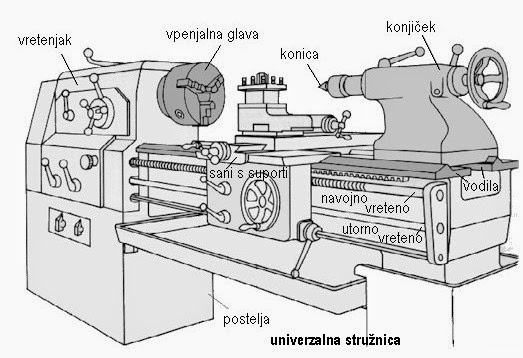
\includegraphics[width=15cm]{deli_struznice.jpg}
        \caption{Glavni deli stružnice
            \cite{deli_struznice}}
        \label{img:deli_struznice}
    \end{center}
\end{figure}

\noindent Glede na glavne dele in njihovo orientacijo in namestitev razlikujemo
predvsem naslednje vrste stružnic:
\begin{itemize}
    \item Univerzalna stružnica (na zgornji sliki [\ref{img:deli_struznice}])
    \item Čelna stružnica
    \item Karoselna stružnica
    \item Revolverska stružnica
\end{itemize}

\noindent Iz navedenih oblik pa so se razvile še posebej specializirane
stružnice kot naprimer:
\begin{itemize}
    \item Kopirna ali podstružilna stružnica
    \item Avtomatska stružnica
    \item Numerično krmiljena stružnica (ali krajše CNC stružnica)
\end{itemize}